\chapter[SCP-146 忏罪铜首]{
    SCP-146 Bronze Head of Shame\\
    SCP-146 忏罪铜首
}

\label{chap:SCP-146}

\begin{figure}[H]
    \centering
    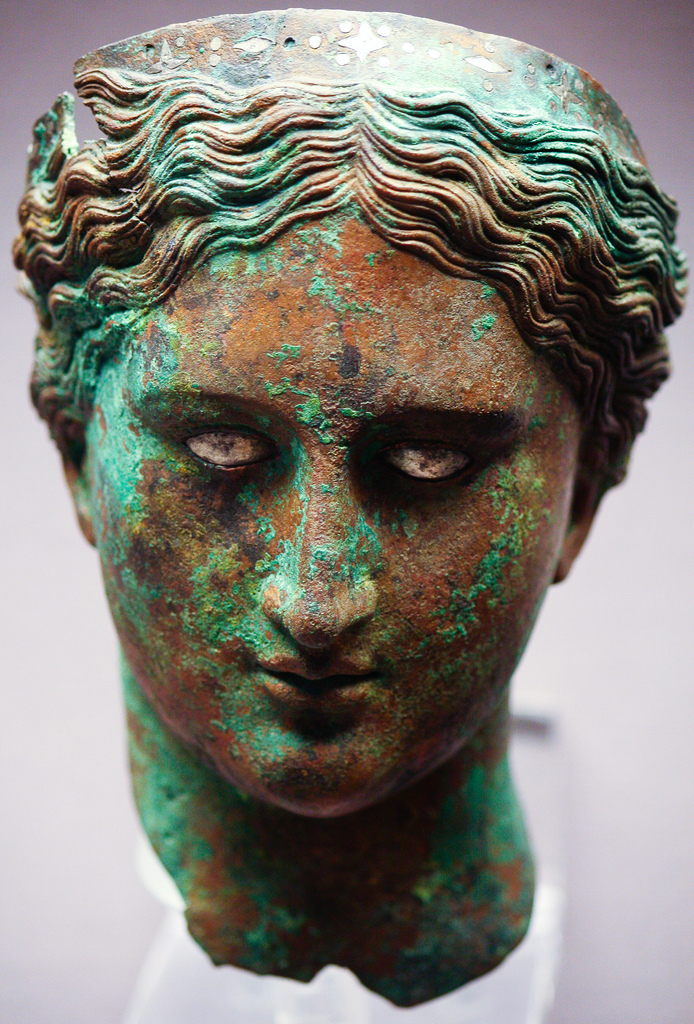
\includegraphics[width=0.5\linewidth]{images/SCP-146.jpg}
    \caption*{注:观察SCP-146的照片被认为是安全的。}
\end{figure}

\bb{项目编号:}SCP-146

\bb{项目等级:}Euclid

\bb{特殊收容措施:}在之前的收容措施(一个标准的半(0.5)米立方体保险容器)中SCP-146的影响正在危险地迅速扩大的情况被指出后,收容程序被修改了。容器应被去除,然而希望测试SCP-146的研究者应处于高度谨慎状态。任何希望将SCP-146装入容器或者遮盖住SCP-146超过两天者都需要3级权限。

在正常存储状况下,SCP-146应被置于其位于{[}数据删除]的储藏室内的一个大理石基座上。SCP-146的标准储藏室尺寸应不小于二十(20)平方米,带有粉刷过的墙壁和一个绘制为晴朗的白昼天空的天花板。房间必须时刻保持明亮(和白昼等效),放置各种盆栽(必须每日照料)并且以罗马共和国晚期(公元前120-公元前80年)的风格装饰。以不同的室内装饰风格进行的实验显示出SCP-146似乎更喜欢这种布置,与那个时代的罗马贵族审美偏好一致。虽然以这种收容方式作为标准,具有二级或者以上权限的研究者可以用不同的收容设置进行试验以改变SCP-146的影响。

尽管SCP-146没有运动能力因此本身只需要低级安保措施,但是任何进入其收容区域或对其进行操作的人员都不能和SCP-146进行目光接触。任何为了避免目光接触而遮盖SCP-146的行为都是被禁止的,因为这已经被证明会以一个不可预测的速率提升SCP-146的影响,一般情况下一(1)天的遮盖或限制会导致SCP-146跳过其影响的初级阶段并直接从最具伤害性的记忆开始。三(3)天之后,SCP-146可以不先进行直接目光接触就产生影响。七(7)天后,SCP-146的影响会变得更加强烈并且不仅限于在SCP-146视野内的对象。在隔壁房间的研究员曾经受到影响,并且其中之一永久性地{[}数据删除]。超过七(7)天的实验在05-█的命令下被否决了。对于必须进入SCP-146的收容区域进行维护的人员提供了眼罩和屏风。

\bb{描述:}SCP-146是一个中空铜首,似乎是一个完整的雕像或胸像的残部,描绘了一个头戴王冠的女性或柔弱的年轻男性。铜像表面大部分都覆盖着严重的铜锈。SCP-146的王冠上镶嵌着银饰,其眼部(SCP-146的影响的表面上的来源)为银箔制成,打磨呈中度反光。目前为止,SCP-146没有显示出任何可以移动的迹象,但是它对它的收容区域中某些装饰的反应显示它就算没有完全的智慧,也具有一定程度的知觉。如果SCP-146能够交流,那么目前为止它尚未这么做。

SCP-146显示出能够读取并且使与其进行直接目光交流者想起某些特定记忆的能力。这些记忆通常与对象的罪恶感和内疚感相联系。经过初步的目光接触后,对象只要停留在SCP-146的视线范围内,记忆和相关感觉就会变得更强烈,而且持续的眼神交流会加速这一过程。

在初次与SCP-146进行眼神交流后,最近的记忆会开始在对象的脑海中浮现。例如曾经在音乐会厅忽略了朋友或者超速的对象会想起这些时间并开始感到些许愧疚,无论他们正常情况下时候会关心这一事件。持续暴露于SCP-146的视线下会导致对象开始想起更久之前也更生动的回忆,同时伴有增加的羞愧感。一般情况下,经过三十(30)分钟的影响后,记忆会从生动的回忆变成强烈的幻象,对象将无法区分过去和现在或者想象和现实。在对象身上也观察到了人格的倒退,尤其是那些回想起童年心理创伤的对象。任何受到影响超过三十分钟的受试者都应该为了他们自身以及其他人的安全被拘束。至今为止所有受SCP-146的影响超过六十(60)分钟的人都完全沉浸在他们的幻觉中;目前这些受试者中无人能从这种紧张性魔怔状态中恢复知觉。此类受试者必须通过静脉注射维持生命并且对外部刺激没有反应,除了偶尔的与他们的悔恨有关的轻声低语。

同样值得注意的是当受试者回想起一个令人愧疚的事件,他们常常会感到自己被迫对他们的行为作出补偿。对于一些轻微的冒犯行为这往往不是问题,并且在某些案例中使员工团结地更紧密。然而,当受试者不能进行补偿时,无论是因为被侵犯的一方无法联系或是犯下了某种不可挽回的罪过,就会产生问题。有时,受试者会致力于进行新的积极正面的努力以“抵消”他们的罪过。然而在大多数这样的案例中,受试者都进入了深度抑郁并且\slash 或者转而进行某种形式的自我惩罚,包括自残和自杀。详情参阅附录实验日志。

SCP-146是从英国伯明翰██████的████先生手中获得的。████先生在已过世的著名慈善家,█████████████勋爵████████ ██████████的身后财产拍卖会上得到了SCP-146,与其他大量工艺品一起以总价█████英镑购得。当████先生开始受到SCP-146的影响,他开始寻求真实身份是特工UA33-56G的心理医生的帮助。███████先生被送进了一个精神病院,SCP-146则被送至基金会保管。UA33-56G对于███████先生的精神状况的笔记被归档为文档SCP-146-A,可供二级及以上研究人员研究。

\hr

\bb{实验记录\#146-01}

一个标准的四(4)米X四(4)米审讯间被一张不透明的幕帘分成两半以测定SCP-146的影响基线。SCP-146被放在房间半边的一张桌子上的有机玻璃防护箱内。在窗帘的另一边受试者D-044323被强行拘束呈直视着SCP-146所在位置的姿势。研究者在整个测试过程中通过对讲机与受试者保持持续联系。

幕帘被去掉,使受试者直接看进了SCP-146的眼睛。受试者的声音立即显出不适并且闭上了眼睛,伴有15BPM的心率上升。在刺激下,受试者讲述了他的记忆,并且开始出现轻微违反常规的行为。对象随后回忆起了在进入基金会之前与其他犯人的争执,包括对{[}DATA REDACTED]特别形象的描述。研究员指出随着时间的推移,受试者变得更加合作并且讲话模式发生了改变,像是一个正在接受催眠治疗的人。

十五(15)分钟以后,受试者的言语变得含糊不清并且他的脑电波波形显示与正在经历一场鲜明梦境的人相似。对象进入了一个进行到一半的对话在他试图冲破拘束时达到了***。经过几分钟,对象停止抽搐并且开始哭泣。对象开始向明显是他幻觉中的某个人乞求:“停下。把它拿回来。不要。我不会再这么做了。我很抱歉。我不想这么做的。不会了。停下……求你……”这种行为一直持续到对象曝露在SCP-146影响下的五十四(54)分钟后,对象的声音停止了并且他的脑电波图显示他昏迷了。又经过一小时后,没有观察到进一步影响,对象被移出并实行了安乐死。对其大脑进行的尸检显示了异常水平的█████████和█████-███████,被神经病理学家█████████描述为{[}数据删除]的象征。

\ii{(注:此时SCP-146是和在拍卖会上得到的其他工艺品存放在一起的,因为当时尚未知晓这种影响仅限于SCP-146拥有。我推定这种收容措施大概是“良好的”收容措施从而将SCP-146的影响归结为其基本的强度。-Skali █████████教授)}

\bb{实验记录\#146-04}\\
确定了SCP-146只包括铜首后设计的第一个实验在SCP-146被转移到一个边长半(0.5)米的立方体储存箱内并在其中存放了两(2)天之后进行。受试者D-044784和SCP-146被置于一个和之前的实验相同的标准审讯室中的幕帘两边。受试者像之前的实验一样被拘束。当幕帘被取下,受试者报告了猛烈迅速的头痛并且开始哭叫。受试者的心率跃升至180BPM但是随后迅速降至40BPM,并且失去了知觉。医护人员进入了房间并且开始检查受试者,这是受试者恢复了知觉,其心率陡升至175BPM。受试者猛烈地试图挣脱拘束,并且很快破坏了右臂的。医护人员D. █████████在受试者为了夺取他的急救箱而攻击他时受了伤。受试者抓起了一把小手术刀并且在守卫重新将其控制住前刺入了她自己的脖颈。医护人员实施了急救,但是受试者在紧急手术时死于失血。

\ii{(注:经过几个类似的事故探明了SCP-146的能力受到其收容措施的影响。任何想做进一步研究的人都应考虑到这一点,因为短暂的意外接触都可能是有害的。-Skali █████████教授)}
